\documentclass[a4paper,12pt]{extarticle}
\usepackage[backend=bibtex]{biblatex}
\addbibresource{mybib.bib}
\usepackage{pgfplots}
\pgfplotsset{compat=1.9}
\usepackage[utf8]{inputenc}
\usepackage[T1,T2A]{fontenc}
\usepackage[english,russian]{babel}
\usetikzlibrary{babel}
\usepackage{graphicx}
\usepackage{wrapfig}
\usepackage{hyperref}
\usepackage{hhline}
\usepackage{multirow}
\usepackage{amsmath,amsfonts,amssymb,amsthm,mathtools}
\usepackage{wasysym}
\usepackage{listings}
\lstset{language=Python}
\usepackage{setspace}
\usepackage[left=1.5cm,right=1.5cm,top=2cm,bottom=2cm]{geometry}
\linespread{1.3}
\usepackage{csquotes}
\usepackage{bchart}
\usepackage{pgf-pie}
\usepackage{tikz}
\usepackage[user,titleref]{zref}
\usepackage{enumitem}
\usetikzlibrary{shadows}
\usepackage{caption}
\usepackage{minted}
\usepackage{subcaption}
\usepackage{multicol}
\usepackage{indentfirst}

\begin{document}

\begin{center}
  \large{\textbf{Тезисы к научно-исследовательской работе <<Алгоритм нахождения наибольшей общей подпоследовательности для нескольких последовательностей Linear-MLCS>>}}
\end{center}

\noindent\textbf{Автор:} Сидюк Дмитрий Андреевич, ученик 11 класса физико-математического профиля Ришельевского научного лицея г. Одесса.

\noindent\textbf{Научный руководитель:} Сидюк Андрей Анатольевич, Senior AI developer (math apparatus), ROMAD Cyber Systems Inc.

\begin{center}
  \line(1,0){450}
\end{center}

\subsection*{Цель}
\vspace{-0.2cm}
Целью данной работы является реализация алгоритма Linear-MLCS на языках программирования Python и C++, а так же исследование некоторых зависимостей в полученных с его помощью последовательностях.

\vspace{-0.5cm}
\subsection*{Актуальность работы}
\vspace{-0.2cm}
Информация в различных своих проявлениях часто выражается в виде последовательностей элементов с конечным алфавитом, что порождает необходимость находить их наибольшие общие подпоследовательности. Будь то цепочка ДНК здорового человека и человека с генетическими отклонениями, паттерны поведения приложений и вредоносных программ, сравнение файлов и т.д. Для решения данной задачи было создано множество алгоритмов. Однако все эти решения объединяет серьезная проблема — они невероятно ресурсозатратные, требуют много памяти и времени для работы.

С современными темпами развития технологий объемы данных стремительно растут, что требует более оптимальных решений проблемы поиска наибольших общих подпоследовательностей. В данной работе будет рассмотрен алгоритм Linear-MLCS, который намного эффективнее аналогов в использовании места и времени необходимого для работы, к тому же он позволяет найти абсолютно все возможные наибольшие общие подпоследовательности \textit{Multiple Longest Common Subsequence} (MLCS) для неограниченного количества последовательностей.

\vspace{-0.5cm}
\subsection*{Ход работы}
\vspace{-0.2cm}
В работе описан принцип действия алгоритма Linear-MLCS на примере последовательностей $S_{1} =$ TFGACGADTC, $S_{2} =$ ATGLCTCAFG и $S_{3} =$ CTADGTALCG с практически выжным в биоинформатике алфавитом, состоящим из обозначений нуклеиновых оснований $\Sigma_{4} = \left\{A, C, G, T\right\}$. Описание разбито на следующте этапы:
\begin{multicols}{2}
  \begin{enumerate}[leftmargin=0.7cm]
    \item Избавление от уникальных элементов
    \item Построение таблиц Successor Tables
    \item Построение NCSG
    \item Сортировка NCSG
    \item Чтение NCSG
    \item[]
  \end{enumerate}
\end{multicols}

На каждом шаге обоснована необходимость данного шага, описан принцип действия, а так же предложена реализация на языках программирования Python и C++. Код программ выложен на GitHub и доступен по ссылке \href{https://github.com/Garison1/MLCS-research}{https://github.com/Garison1/MLCS-research}.

\subsection*{Итоги исследования}
За время выполнения работы мы реализовали алгоритм Linear-MLCS на языках программирования Python и C++, в том числе метод построения NCSG графа, его чтения, а так же методы прямой и обратной топологических сортировок. Описали работу алгоритма на примере его реализации на языке Python. Провели исследования зависимостей количества полученных LCS от их длины, определили распределение вероятностей длин LCS и их количества. \nocite{1}

\printbibliography[heading=subbibintoc]

\subsection*{\textbf{Приложения}}

\centerline{\textbf{Приложение 1: }Построенные Successor Tables для последовательностей $S_{1}$, $S_{2}$ и $S_{3}$}
\begin{table}[h!]
  \centering
  \renewcommand{\arraystretch}{1.5}
  \renewcommand{\tabcolsep}{0.25cm}
  \begin{tabular}{ c | c | c | c | c | c | c | c | c | c |}
    $S_{1}$ & $=$ & T & G & A & C & G & A & T & C \\
            & 0 & 1 & 2 & 3 & 4 & 5 & 6 & 7 & 8 \\
    \hline
    A & 3 & 3 & 3 & 6 & 6 & 6 & - & - & - \\
    \hline
    C & 4 & 4 & 4 & 4 & 8 & 8 & 8 & 8 & - \\
    \hline
    G & 2 & 2 & 5 & 5 & 5 & - & - & - & - \\
    \hline
    T & 1 & 7 & 7 & 7 & 7 & 7 & 7 & - & - \\
    \hline
  \end{tabular}
\end{table}
\begin{table}[h!]
  \hspace{-1.5cm}
  \centering
  \renewcommand{\arraystretch}{1.5}
  \renewcommand{\tabcolsep}{0.25cm}
  \begin{tabular}{ c | c | c | c | c | c | c | c | c | c |}
    $S_{2}$ & $=$ & A & T & G & C & T & C & A & G \\
            & 0 & 1 & 2 & 3 & 4 & 5 & 6 & 7 & 8 \\
    \hline
    A & 1 & 7 & 7 & 7 & 7 & 7 & 7 & - & - \\
    \hline
    C & 4 & 4 & 4 & 4 & 6 & 6 & - & - & - \\
    \hline
    G & 3 & 3 & 3 & 8 & 8 & 8 & 8 & 8 & - \\
    \hline
    T & 2 & 2 & 5 & 5 & 5 & - & - & - & - \\
    \hline
  \end{tabular}\hspace{1cm}
  \begin{tabular}{ c | c | c | c | c | c | c | c | c | c |}
    $S_{3}$ & $=$ & C & T & A & G & T & A & C & G \\
            & 0 & 1 & 2 & 3 & 4 & 5 & 6 & 7 & 8 \\
    \hline
    A & 3 & 3 & 3 & 6 & 6 & 6 & - & - & - \\
    \hline
    C & 1 & 7 & 7 & 7 & 7 & 7 & 7 & - & - \\
    \hline
    G & 4 & 4 & 4 & 4 & 8 & 8 & 8 & 8 & - \\
    \hline
    T & 2 & 2 & 5 & 5 & 5 & - & - & - & - \\
    \hline
  \end{tabular}
  \hspace{-1.5cm}
\end{table}
\clearpage
\begin{figure}[h!]
  \vspace{-1cm}
  \centering
  \caption*{\textbf{Приложение 2: }Построенный \textit{Non-redundant Common Subsequence Graph} (NCSG)}
  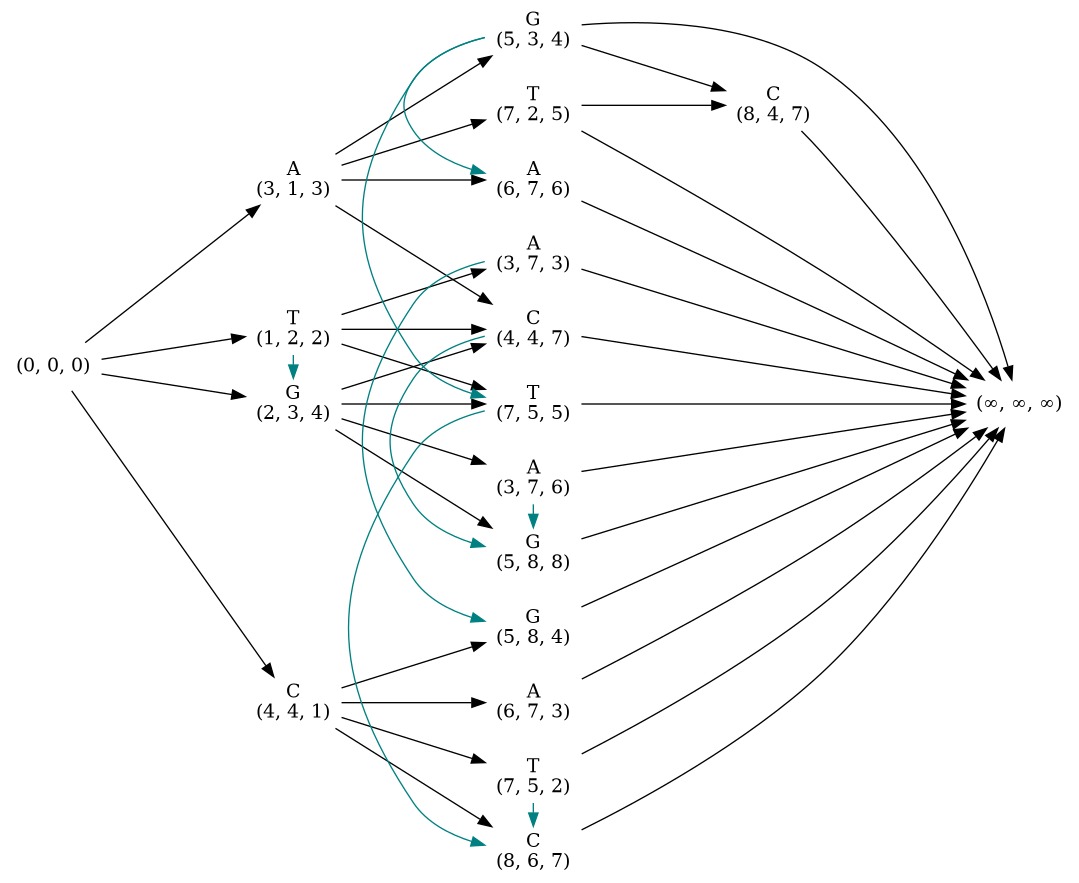
\includegraphics[width=0.7\textwidth]{Graph_1.png}
\end{figure}

\begin{figure}[h!]
  \centering
  \caption*{\textbf{Приложение 3: }NCSG отсортированный прямой топологической сортировкой}
  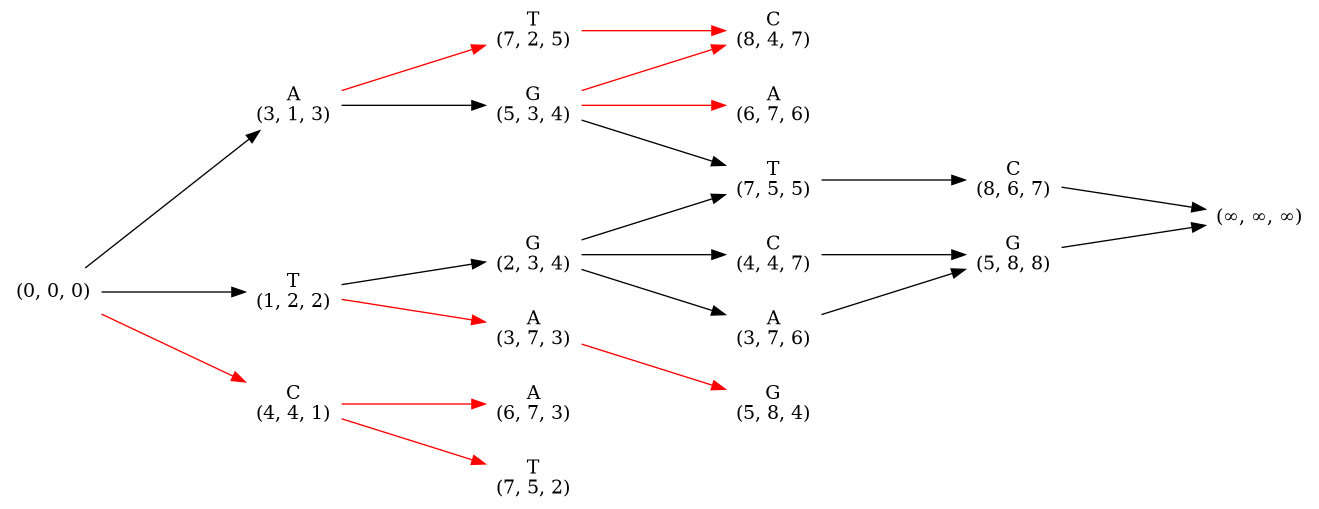
\includegraphics[width=1\textwidth]{Graph_2.png}
\end{figure}

\begin{figure}[h!]
  \caption*{\textbf{Приложение 4: }NCSG отсортированный обратной топологической сортировкой}
  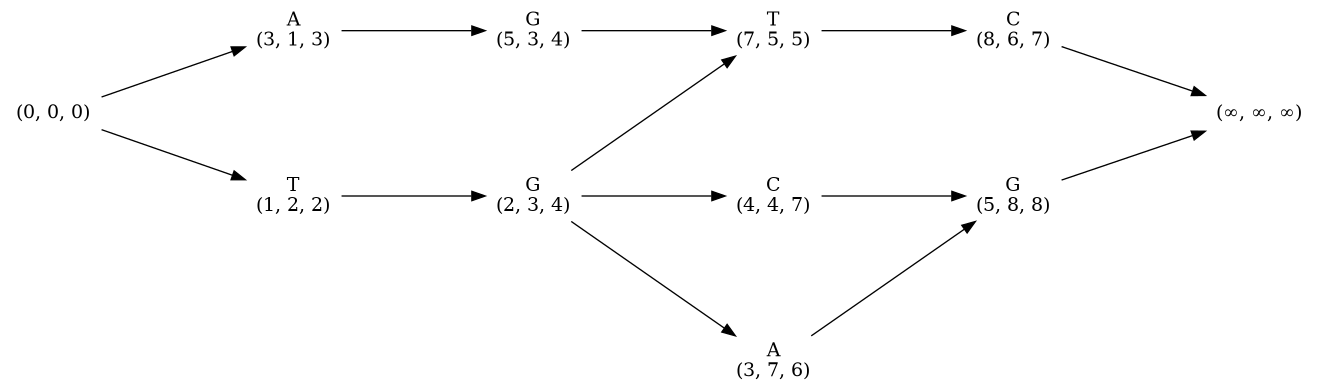
\includegraphics[width=1\textwidth]{Graph_3.png}
  \vspace{-3cm}
\end{figure}
\clearpage

\begin{figure}[h!]
  \caption*{\textbf{Приложение 5: }Гистограмма вероятностей количества LCS}
  \label{fig:1}
  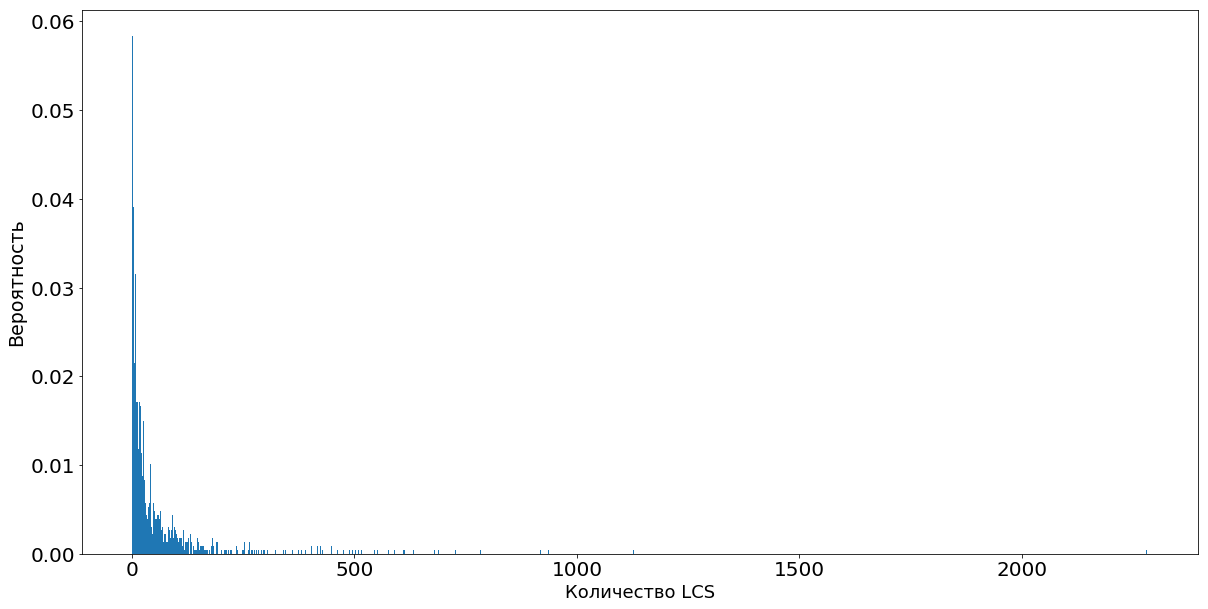
\includegraphics[width=1\textwidth]{Diogram_1.png}
  \centering
  \begin{subfigure}{.5\textwidth}
    \vspace{1.5cm}
    \centering
    \captionsetup{justification=centering}
    \caption*{\textbf{Приложение 6: }Соотношение между длинами\\получаемых LCS и их количеством.}
    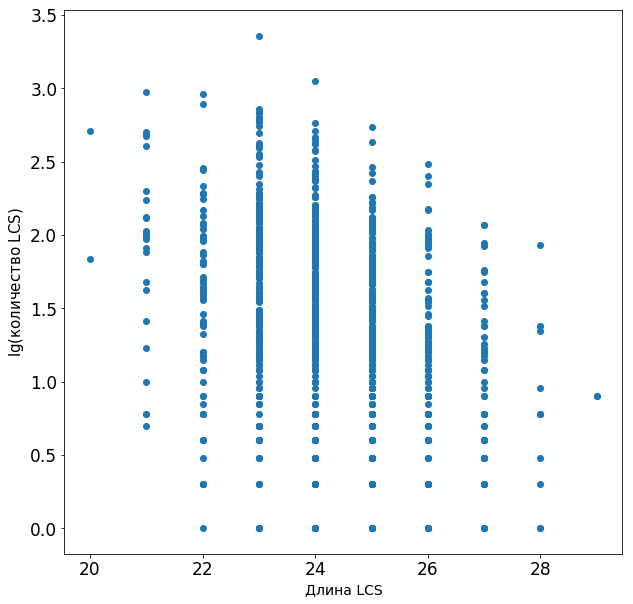
\includegraphics[width=0.9\textwidth]{Diogram_2.png}
    \label{fig:2}
  \end{subfigure}%
  \begin{subfigure}{.5\textwidth}
    \vspace{1.5cm}
    \centering
    \captionsetup{justification=centering}
    \caption*{\textbf{Приложение 7: }Гистограмма распределения\\вероятностей длин LCS}
    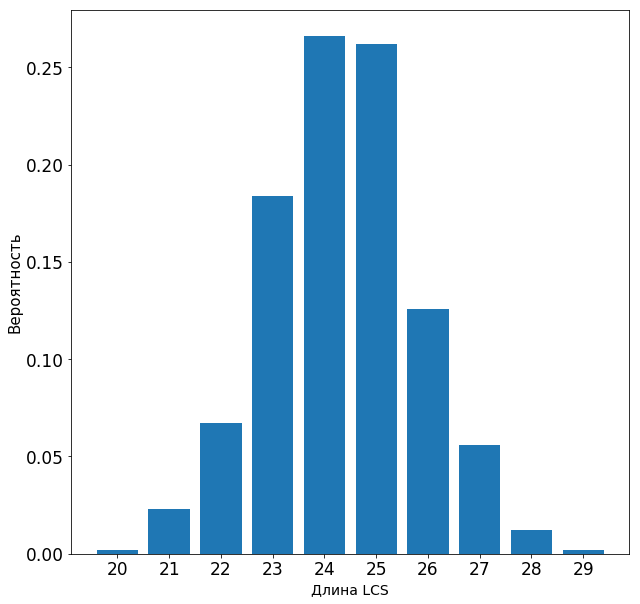
\includegraphics[width=0.9\textwidth]{Diogram_3.png}
    \label{fig:3}
  \end{subfigure}
\end{figure}
\textbf{Примечание: } На приложениях \hyperref[fig:1]{5}, \hyperref[fig:2]{6} и \hyperref[fig:3]{7} изображены диограммы, полученные после анализа 1000 наборов из 3 последовательностей длиной 50 элементов и алфавитом 4.
\end{document}


% Local Variables:
% LaTeX-command: "latex -shell-escape"
% End:
